\part{Constraint Solving and Abstraction}


\chapter{Constraint Solving}


\section{Symbolic Execution and SMT Solving}\label{sec:se-smt}

As mentioned \autoref{sec:satisfiability-and-activation-pattern-search}, the DNN verification problem can be represented as a satisfiability problem as shown in~\autoref{eq:prob}.  Specifically, we can encode the DNN as a logical formula and use an SMT solver to check that it satisfies the property of interest.

A straightforward way to do this encoding is using \emph{symbolic execution} (SE)~\cite{FIXME}, a well-known software testing technique for finding bugs.  SE executes a program on symbolic inputs, i.e., inputs represented as symbols rather than concrete values, and tracks the reachability of program state as symbolic expressions, i.e., logical formulae over symbolic inputs. The satisfiability of these formulae is then checked using an SMT solver, and satisfying assignments represent inputs leading to the undesirable (buggy) program state.

\subsection{Symbolic Execution}\label{sec:se}
We can adapt traditional SE to our problem by treating the DNN as a program and neurons as variables and executing the DNN on symbolic inputs. Affine transformations can easily be represented as logical formulae because they are linear functions. Activation functions such as ReLUs are translated to disjunctions of linear functions or if-then-else statements, i.e., $ReLU(x) = \max(x,0) \equiv x \ge 0 \land x \lor 0 \land \neg x$.


For example, for the DNN in \autoref{fig:dnn}, we can symbolically execute the DNN on symbolic inputs $x_1,x_2$ and return the symbolic output $x_5$ as 

\begin{equation}
    \begin{split}
x_5 &= -x_3 + x_4 - 1 ~\land \\
x_3 &= \max(-0.5x_1 + 0.5x_2 + 1.0, 0) ~\land \\
x_4 &= \max(0.5x_1 - 0.5x_2 - 1.0, 0)
    \end{split}
\end{equation}


\subsection{SMT Solving}\label{sec:smt}
We can then use an SMT solver to check that the formula $x_5 \le 0$ is satisfiable for any inputs $x_1 \in [-1,1], x_2\in[-2,2]$.


\subsection{Limitations}\label{sec:smt-limitations} 
%mention the work that treat DNN as a Java program and apply JPF.  
\section{MILP}

As mentioned in~\autoref{sec:smt-limitations}, using a generic, off-the-shelf SMT solver to verify DNNs can be inefficient because the computed formulae can be large and complex due to disjunctions representing non-linear activation functions.  This can lead to an explosion in the number of paths to explore, especially for large DNNs with many neurons.
To address this, we can use a Mixed Integer Linear Programming (MILP) solver, which is specialized for solving linear constraints and is more efficient for DNN verification. Indeed, many modern DNN verification tools~\cite{wang2018efficient,katz2017reluplex,henriksen2020efficient} use industrial-strength MILP solvers such as Gurobi to help verify DNNs.

We can encode the DNN as a set of linear constraints and use an MILP solver to check that the constraints are satisfiable. For example, the DNN in \autoref{fig:dnn} can be encoded as a set of linear constraints as follows:\tvn{Hai, fill out this section on MILP}


\subsubsection{Limitations}\label{sec:milp-limitations}



\chapter{Abstraction}

\section{Interval}

An interval abstraction is a simple and widely-used abstraction technique in DNN verification. It estimates the over-approximated range of values that a neuron can take using a lower and upper bound $[l, u]$. An interval $[l, u]$ denotes the potential set.
$$\{x \ | \ l \leq x \leq u\}$$

From here, we can define a set of functions commonly appearing in the neural network that can operate on an interval.

\subsection{Affine functions}

For affine function \(f\) in \ref{sec:affine}
\[f(v_1, v_2, ...,v_n) = \sum_{i}^{n}w_iv_i\]
where $n$ is number of output nodes from the previous layer. We can define the abstract transformer \(f^a\) as follows:
\[f^{a}([l_1, u_1],...,[l_n, u_n]) = [w^+\cdot l + w^- \cdot u, w^+ \cdot u + w^- \cdot l]\]

where \(l \in \mathbb{R}^n\) and \(u \in \mathbb{R}^n\) represent the lower \([l_1, l_2, ... l_n]\) and upper bounds \([u_1, u_2, ... u_n]\) of the nodes of the previous layer respectively, \(w^+\) included positive weight values while \(w^-\) included negative ones, following these equations:

\[
w^+_i =
\begin{cases}
w_i, & \text{if } w_i > 0 \\
0, & \text{otherwise}
\end{cases}
\quad \text{for } i = 1, 2, \dots, n
\]

\[
w^-_i =
\begin{cases}
w_i, & \text{if } w_i \leq 0 \\
0, & \text{otherwise}
\end{cases}
\quad \text{for } i = 1, 2, \dots, n
\]

\subsection{Activation Functions}

Most activation functions used in neural networks are monotonically increasing, e.g., ReLU and sigmoid. It is straightforward to define
an abstract transformer for any monotonically increasing function \(f : \mathbb{R} \to \mathbb{R}\), as we simply apply \(f\) for lower and upper bounds as follows:
\[f^a
([l, u]) = [ f(l), f(u)]
\]

The interval abstraction is efficient and easy to implement, but it can be imprecise, especially for non-linear activation functions like ReLU. 

\paragraph{Example}: For the DNN in \autoref{fig:dnn}, the interval abstraction for the input layer is $x_1 \in [-1, 1]$ and $x_2 \in [-2, 2]$. The interval abstraction for the hidden layer is $x_3 \in [0, 2]$ because $x_3 = [ReLU(-0.5x_1 + 0.5x_2 + 1.0), ReLU(-0.5x_1 + 0.5x_2 + 1.0)] = [ReLU(-0.5 \times -1 + 0.5 \times -2 + 1.0), ReLU(-0.5 \times 1 + 0.5 \times 2 + 1.0)] = [0, 2]$. Similarly, $x_4 \in [0, 2]$. The interval abstraction for the output layer is $x_5 \in [-3, 3]$.

\section{Zonotope}

\section{Zonotope Abstraction for DNN Verification}

Zonotope abstraction is a more precise technique than interval abstraction for verifying the behavior of deep neural networks (DNNs). Unlike interval abstraction, which considers each variable independently, zonotopes capture correlations between variables (e.g., neuron activations), thereby reducing over-approximation errors in the verification process.

\subsection{Definition of a Zonotope}

A \textbf{zonotope} is a geometric object that can be viewed as the result of applying an affine transformation to a high-dimensional cube. Formally, a zonotope \(\mathcal{Z}\) in \(\mathbb{R}^n\) is defined as:

\[
\mathcal{Z} = \left\{c + \sum_{i=1}^{m} \epsilon_i g_i \mid \epsilon_i \in [-1, 1]\right\}
\]

where:
\begin{itemize}
    \item \(c \in \mathbb{R}^n\) is the \textit{center} of the zonotope,
    \item \(g_i \in \mathbb{R}^n\) are called \textit{generator vectors},
    \item \(m\) is the number of generators,
    \item \(\epsilon_i\) are independent scalar coefficients bounded between \(-1\) and \(1\).
\end{itemize}

This representation means that the zonotope contains all points that can be formed by adding scaled versions of the generator vectors to the center. The coefficients \(\epsilon_i\) determine the range of influence each generator has.

\paragraph{Example (1D)} Consider a one-dimensional case with \(n = 1\), one generator (\(m = 1\)), and scalar center and generator:

\[
\mathcal{Z} = \left\{c + \epsilon_1 g_1 \mid \epsilon_1 \in [-1, 1]\right\}
\]

This is simply the interval \([c - g_1, c + g_1]\).

\paragraph{Example (2D)} To illustrate zonotopes in higher dimensions, suppose:

\[
c = \begin{bmatrix}2 \\ 3\end{bmatrix}, \quad
g_1 = \begin{bmatrix}1 \\ 1\end{bmatrix}
\]

Then, the set:

\[
\left\{c + \epsilon_1 g_1 \mid \epsilon_1 \in [-1, 1]\right\}
= \left\{
\begin{bmatrix}2 + \epsilon_1 \\ 3 + \epsilon_1\end{bmatrix}
\right\}
\]

describes a line segment between \((1, 2)\) and \((3, 4)\).

Now add a second generator:

\[
g_2 = \begin{bmatrix}0 \\ 1\end{bmatrix}
\]

The zonotope becomes:

\[
\left\{
\begin{bmatrix}2 \\ 3\end{bmatrix} + \epsilon_1 \begin{bmatrix}1 \\ 1\end{bmatrix} + \epsilon_2 \begin{bmatrix}0 \\ 1\end{bmatrix}
\mid \epsilon_1, \epsilon_2 \in [-1, 1]
\right\}
= \left\{
\begin{bmatrix}2 + \epsilon_1 \\ 3 + \epsilon_1 + \epsilon_2\end{bmatrix}
\right\}
\]

This forms a parallelogram in 2D space. As more generators are added, the shape becomes more complex, and the zonotope can approximate more intricate geometric regions.

\begin{figure}[h]
    \centering
    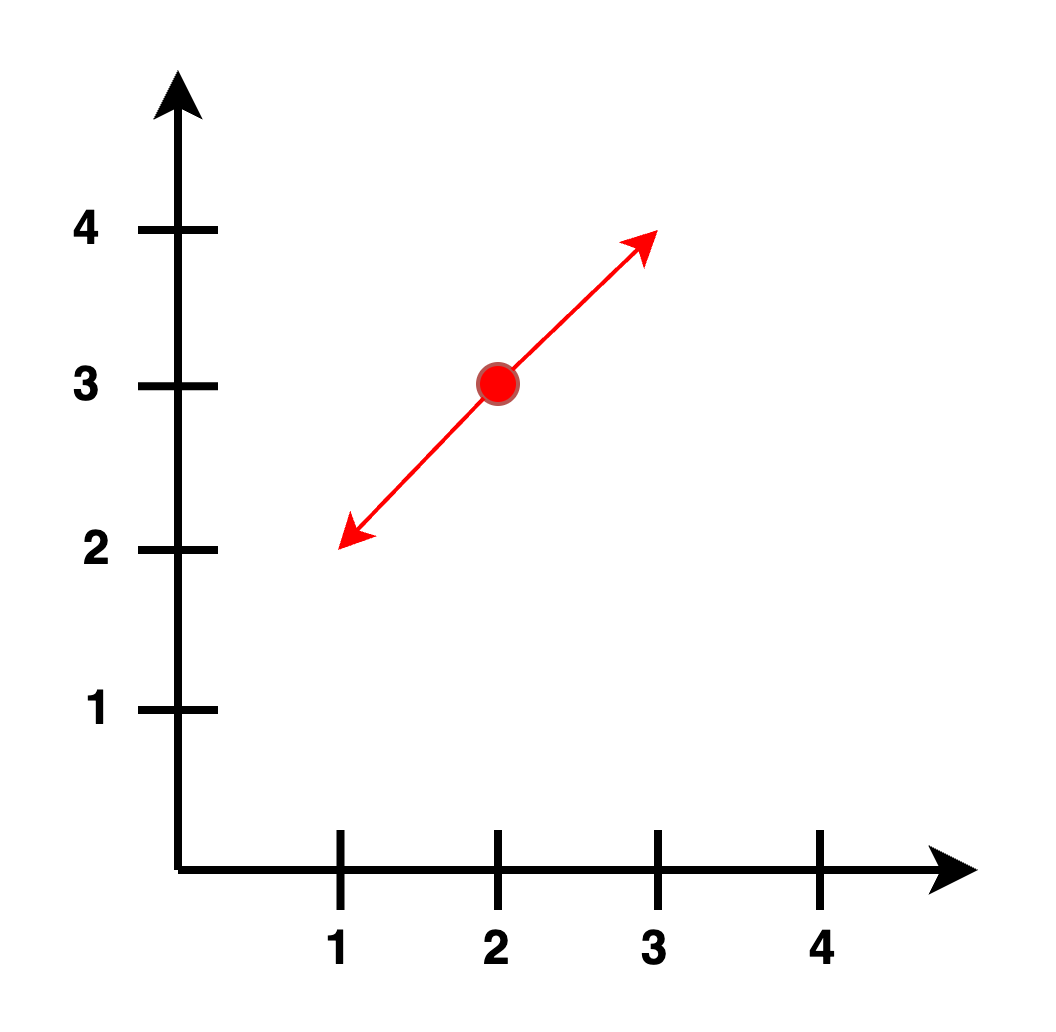
\includegraphics[width=0.5\linewidth]{figure/2d-zonotope.png}
    \caption{Illustration of a 2D zonotope with increasing number of generators.}
    \label{fig:zonotope-example}
\end{figure}

\subsection{Affine Transformations}

Zonotopes are closed under affine transformations, which makes them especially useful for modeling the linear layers of neural networks.

An affine function is of the form:

\[
f(x) = W x + b
\]

where \(W\) is a weight matrix and \(b\) is a bias vector. Given a zonotope \(\mathcal{Z} = (c, G)\), where \(G\) is a matrix whose columns are the generator vectors \(g_i\), we define the abstract transformer:

\[
f^a(\mathcal{Z}) = (Wc + b, WG)
\]

This means:
\begin{itemize}
    \item The new center is \(Wc + b\),
    \item The new generator matrix is \(WG\), where \(W\) is applied to each generator.
\end{itemize}

Since affine functions preserve the zonotope structure, no over-approximation is introduced at this stage.

\subsection{Non-Linear Activation Functions}

Activation functions such as ReLU are not affine and therefore do not preserve the zonotope structure. To handle them, conservative approximations are used.

\paragraph{ReLU Relaxation:} Suppose a neuron has input represented as a zonotope, and we apply the ReLU function \(\text{ReLU}(x) = \max(0, x)\). There are two cases:

\begin{itemize}
    \item \textbf{Non-negative range:} If all possible values of the neuron (based on the zonotope) are non-negative, ReLU acts linearly and is applied directly.
    \item \textbf{Mixed range:} If the range of values crosses zero, we must over-approximate. A common method is to introduce new generator vectors or define upper and lower affine bounds to contain the output.
\end{itemize}

This relaxation is necessary to ensure soundness (i.e., all real behaviors are contained), but it introduces some loss of precision.

\paragraph{Example:} Let the input zonotope be:

\[
\mathcal{Z}_{\text{input}} = (c, G), \quad
c = \begin{bmatrix} 0 \\ 0 \end{bmatrix}, \quad
G = \begin{bmatrix} 1 & 0 \\ 0 & 2 \end{bmatrix}
\]

This describes the domain:
\[
x_1 \in [-1, 1], \quad x_2 \in [-2, 2]
\]

Now consider the ReLU layer:

\[
x_3 = \text{ReLU}(-0.5x_1 + 0.5x_2 + 1.0)
\]
\[
x_4 = \text{ReLU}(0.5x_1 - 0.5x_2 + 1.0)
\]

First, apply the affine transformation:

\[
\mathcal{Z}_{\text{affine}} = (Wc + b, WG)
\]

Next, check whether each component's range crosses zero. If it does, use ReLU relaxation techniques such as:

\begin{itemize}
    \item \textbf{DeepZ} – introduces extra generators to improve precision,
    \item \textbf{AI\(^2\)} – uses zonotope splitting for tighter bounds.
\end{itemize}

After relaxation, apply the next affine transformation to complete the forward pass.

\subsection{Comparison with Interval Abstraction}

Interval abstraction represents each neuron as an independent interval \([a_i, b_i]\). While simple and fast, it loses inter-variable relationships, leading to large over-approximation errors, especially in deeper networks.

In contrast, zonotopes retain dependencies between neurons via shared generators, providing tighter bounds and better scalability. However, they come at the cost of increased complexity, especially when dealing with non-linear operations.

\paragraph{Summary:}
\begin{itemize}
    \item \textbf{Interval abstraction} is simple but imprecise.
    \item \textbf{Zonotope abstraction} is more precise and scalable, particularly effective for networks with affine layers.
    \item \textbf{Non-linear activations} introduce challenges, requiring trade-offs between precision and computational overhead.
\end{itemize}



\section{Polytope}

In the previous section, we have seen the abstract domain of zonotopes, which is more expressive than the interval domain. Specifically, instead of approximating functions using a hyper-rectangle, the zonotope domain allows us to approximate functions using a zonotope, e.g., a parallelogram, capturing relations between different dimensions. In this section, we look at an even more expressive abstract domain, the polyhedron (or polytope) domain. 

Unlike the zonotope domain, the polyhedron domain allows us to approximate functions using arbitrary convex polyhedra. A polyhedron in \(\mathbb{R}^n\) is a region made of straight (as opposed to curved) faces; a convex shape is one where the line between any two points in the shape is completely contained in the shape. Convex polyhedra can be specified as a set of linear inequalities of the form:

\[
Ax \leq b
\]

where \(A \in \mathbb{R}^{m \times n}\) and \(b \in \mathbb{R}^m\) for some \(m\), specifying \(m\) half-spaces whose intersection forms the polyhedron.

Using a set of convex polyhedra, we can more precisely approximate activation functions like ReLU. For instance, to approximate ReLU, we can describe the tightest convex over-approximation by the following constraints:

\[
x \leq y, \quad 0 \leq y, \quad y \leq \lambda x + \mu
\]

where \(\lambda\) and \(\mu\) are parameters chosen based on the bounds of \(x\).

\begin{figure}[h]
    \centering
    \includegraphics[width=0.5\linewidth]{figure/3-lines-polytope.png}
    \caption{The tightest Convex Polyhedral Approximation of ReLU.}
    \label{fig:enter-label}
\end{figure}
% \begin{figure}
%     \centering
%     \includegraphics[width=0.5\linewidth]{3-lines-polytope.png}
%     \caption{Enter Caption}
%     \label{fig:enter-label}
% \end{figure}

This is the smallest convex polyhedron that soundly approximates ReLU, and is strictly more precise than the interval and zonotope abstractions, as can be seen visually.

\subsection{Affine Functions}

Affine transformations map convex polyhedra to convex polyhedra.  
Given an affine transformation \(f(x) = Wx + b\), where \(W\) is a matrix and \(b\) is a bias vector, we can transform a polyhedron \(\{x \mid A x \leq b\}\) through \(f\) by substitution:

\[
\{x \mid A (W^{-1}(x - b)) \leq b\}
\]

if \(W\) is invertible. More commonly in practice, when applying affine transformations in neural networks (layer-wise), we modify the constraints accordingly by propagating through the weights and biases.

Thus, affine layers can be handled exactly under polyhedral abstraction without any need for relaxation or over-approximation.

\subsection{Activation Functions}

Handling non-linear activation functions, such as ReLU, with polyhedral abstraction is challenging because non-linearities generally map polytopes to non-convex shapes. Therefore, over-approximations are required.

The key idea is to approximate the graph of the non-linear function by a convex polyhedron that covers all possible cases. For ReLU, the previously mentioned three constraints:

\begin{equation}\label{minimum_polyhedron}
x \leq y, \quad 0 \leq y, \quad y \leq \lambda x + \mu
\end{equation}


construct a tight convex relaxation.

For other activations like sigmoid or tanh, the approximation involves linearizing the curve between the lower and upper bounds of the input variable, but the number of constraints can quickly grow, increasing computational complexity.

\paragraph{DeepPoly.}  
By containing two lower polyhedra constraints for \(y\), the approximation in \ref{minimum_polyhedron} inherently suffers from a potential blow-up in number of constraints as the analysis proceeds. Due to scalability issues associated with general polyhedral representations, DeepPoly \cite{singh2019abstract} was proposed as a precise and scalable abstract domain. DeepPoly introduces a specialized form of polyhedral abstraction combined with interval bounds. 

More specifically,  DeepPoly only allows for one lower bound in \ref{minimum_polyhedron}, the selection of which lower constraint depends on which constraint provides the tighter approximation.

Returning to our example, the area of the approximation in Fig.~4(b) is given by \( 0.5 \cdot u \cdot (u - l) \), while the area in Fig.~4(c) is given by \( 0.5 \cdot (-l_i) \cdot (u_i - l_i) \). To achieve a tighter relaxation, we select the approximation with the smaller area. Specifically, when \( u \leq -l \), we apply the constraints and bounds derived from \(x \leq y\).
In addition, each neuron \(x_j\) is bounded above and below by affine expressions of the input neurons:

\[
l_j(x) \leq x_j \leq u_j(x)
\]

where \(l_j\) and \(u_j\) are affine functions.

\subsection{DeepPoly Transformers}

The DeepPoly abstract domain defines a scalable and precise framework for verifying deep neural networks by combining interval and polyhedral abstractions. Each neuron is bounded from above and below using affine expressions of the input neurons:

\[
l_j(x) \leq x_j \leq u_j(x)
\]

where \(l_j(x)\) and \(u_j(x)\) are affine functions representing lower and upper bounds respectively. DeepPoly then defines **abstract transformers** to propagate these bounds through different types of neural network layers.

\subsubsection{Affine Layer Transformer}

Given an affine transformation:
\[
x^{(l+1)} = W x^{(l)} + b
\]

we define the transformation of the bounds by propagating the affine expressions directly:
\begin{align*}
l_j^{(l+1)}(x) &= \sum_i w_{ji}^+ \cdot l_i^{(l)}(x) + w_{ji}^- \cdot u_i^{(l)}(x) + b_j \\
u_j^{(l+1)}(x) &= \sum_i w_{ji}^+ \cdot u_i^{(l)}(x) + w_{ji}^- \cdot l_i^{(l)}(x) + b_j
\end{align*}

Here, \(w^+_{ji} = \max(w_{ji}, 0)\), and \(w^-_{ji} = \min(w_{ji}, 0)\), ensuring correct handling of sign-dependent propagation.

\subsubsection{ReLU Transformer}

The ReLU transformer in DeepPoly uses a convex relaxation that is tighter than previous abstractions by selecting only one lower bound constraint depending on the sign and tightness. Suppose \(x_j = \text{ReLU}(x_i)\). Let \([l_i, u_i]\) be the lower and upper bounds for \(x_i\).

\begin{itemize}
    \item If \(l_i \geq 0\): ReLU is linear, so
    \[
    l_j(x) = l_i(x), \quad u_j(x) = u_i(x)
    \]

    \item If \(u_i \leq 0\): ReLU is constant 0, so
    \[
    l_j(x) = u_j(x) = 0
    \]

    \item If \(l_i < 0 < u_i\): ReLU is approximated with:
    \[
    u_j(x) = \frac{u_i}{u_i - l_i} \cdot (x_i - l_i)
    \]
    and only one lower bound is selected:
    \[
    l_j(x) =
    \begin{cases}
        0, & \text{if area under lower 0 line is smaller} \\
        x_i, & \text{if area under identity line is smaller}
    \end{cases}
    \]
\end{itemize}

The decision is made based on which convex region has smaller area to achieve a tighter abstraction, following the principle:
\[
\text{Choose constraint with smaller area:} \quad 0.5 \cdot u_i \cdot (u_i - l_i) \quad \text{vs} \quad 0.5 \cdot (-l_i) \cdot (u_i - l_i)
\]


By maintaining only upper and lower affine bounds, DeepPoly avoids the full complexity of manipulating arbitrary polytopes while retaining significantly more precision than intervals or zonotopes. 

...

Thus, DeepPoly achieves a practical balance between precision and scalability for verifying deep neural networks.

\subsection{Example}

Consider again the DNN in \autoref{fig:dnn}. Suppose the input set is defined by box constraints \(x_1 \in [-1,1]\) and \(x_2 \in [-2,2]\). These can be represented initially by 4 inequalities.

Applying the affine transformation for the hidden layer, we obtain a new set of inequalities describing the hidden layer nodes. Upon applying ReLU, we would use the convex polyhedral relaxation as depicted in \autoref{fig:3_lines_polytope}. The output layer similarly results from affine operations on the polyhedra describing the hidden layer.

In a DeepPoly setting, instead of carrying full inequalities, we track only the lower and upper affine bounds per neuron, leading to an efficient verification process.

\subsection{Comparison to Zonotope Abstraction}

While zonotope abstraction captures dependencies between variables better than intervals, it still assumes symmetrical dependencies around a center point and cannot easily model arbitrary convex shapes.

Polyhedral abstraction, on the other hand, allows representing arbitrary convex shapes precisely, enabling much tighter approximations, especially after ReLU activations.

However, traditional polyhedral methods suffer from:
\begin{itemize}
    \item High computational complexity,
    \item Rapid growth in the number of constraints,
    \item Difficulty scaling to large networks.
\end{itemize}

DeepPoly addresses these challenges by:
\begin{itemize}
    \item Restricting to simple upper and lower affine bounds,
    \item Maintaining polynomial scalability,
    \item Achieving higher precision than zonotopes or intervals,
    \item Providing efficient transformers for common layers in DNNs.
\end{itemize}

Therefore, DeepPoly achieves a balance, combining the expressiveness of polyhedral domains with the efficiency required for deep network verification.



